\documentclass[12pt,letterpaper]{exam}
\usepackage[lmargin=1in,rmargin=1in,tmargin=1in,bmargin=1in]{geometry}
\usepackage{../style/exams}

% -------------------
% Course & Exam Information
% -------------------
\newcommand{\course}{MAT 308: Exam 3}
\renewcommand{\term}{Fall -- 2022}
\newcommand{\examdate}{12/15/2022}
\newcommand{\timelimit}{`$\infty$' Minutes}

\setbool{hideans}{true} % Student: True; Instructor: False

% -------------------
% Content
% -------------------
\begin{document}

\examtitle
\instructions{Write your name on the appropriate line on the exam cover sheet. This exam contains \numpages\ pages (including this cover page) and \numquestions\ questions. Check that you have every page of the exam. Answer the questions in the spaces provided on the question sheets. Be sure to answer every part of each question and show all your work. If you run out of room for an answer, continue on the back of the page --- being sure to indicate the problem number.} 
\scores
\bottomline
\newpage

% ---------
% Questions
% ---------
\begin{questions}

% Question 1
\newpage
\question[10] Define the following vectors and matrices:
	\[
	u= \begin{pmatrix} 1 \\ 0 \\ -2 \end{pmatrix}, \quad
	v= \begin{pmatrix} 5 \\ -1 \\ 6 \end{pmatrix}, \quad
	A= \begin{pmatrix} 1 & 0 & 1 \\ 1 & 1 & 0 \\ 0 & 0 & 1 \end{pmatrix}, \quad
	B= \begin{pmatrix} 1 & 0 & 1 \\ 2 & -1 & 0 \\ 0 & 3 & 5 \\ -1 & 0 & 1 \end{pmatrix}, \quad
	C= \begin{pmatrix} 2 & -1 & 0 \\ -4 & 3 & 7 \\ 6 & 11 & 8 \end{pmatrix}
	\]
Showing all your work and fully justifying your responses, answer the following:
	\begin{enumerate}[(a)]
	\item Compute $-5u - 2v$.
	\item Compute $u \cdot v$.
	\item Compute $A^2$.
	\item Compute $Bu$
	\item Consider $BC$ and $CB$. If the product is not defined, explain why. If the product is defined, compute it. 
	\end{enumerate}



% Question 2
\newpage
\question[10] Suppose that $A$, $B$, $C$, and $D$ are events in a finite probability space. Define the following probabilities:
	\[
	\begin{aligned}
	P(A)&= 0.24 & P(B \;|\; A)&= 0.90 \\
	P(B)&= 0.61 & P(C \cap D)&= 0 \\
	P(C)&= 0.15 \\
	P(D)&= 0.86
	\end{aligned}
	\]
Showing all your work and fully justifying your responses, answer the following:
	\begin{enumerate}[(a)]
	\item What is $P(A^c)$?
	\item Are $A^c$ and $D$ disjoint? Explain. 
	\item Assuming $B$ and $C$ are independent, compute $P(B \cup C)$.
	\item Compute $P(A \cap B)$.
	\item Are $A$ and $B$ independent? Explain. Are $C$ and $D$ independent? Explain.
	\end{enumerate}



% Question 3
\newpage
\question[10] Showing all your work and fully justifying your reasoning, answer the following:
	\begin{enumerate}[(a)]
	\item How many arrangements of letters are there using the letters from the word `trichotillomania'?
	\item How many arrangements of letters are there using the letters from `assessment' such that `a' and `t' appear alphabetically with 5 letters between them?
	\item How many 4 character passwords with exactly one vowel can be formed using only English lower case letters and no repeated letters?
	\item How many ways are there of breaking a room with 10 students into three groups with size five, three, and two, respectively. 
	\end{enumerate}



% Question 4
\newpage 
\question[10] Showing all your work and fully justifying your reasoning, answer the following:
	\begin{enumerate}[(a)]
	\item How many combinations of 15 chicken wings can be ordered at a restaurant that offers 20 different flavors of wings? 
	\item How many integer solutions are there to $x_1 + x_2 + x_3= 20$ with $x_1, x_2, x_3 \geq 1$?
	\item What is the coefficient of $x^{12} y^8$ in $\left( 5y - \dfrac{x}{2} \right)^{20}$?
	\item What is the coefficient of $x^3 y^2 z^5$ in $(x + y - z)^{10}$?
	\end{enumerate}



% Question 5
\newpage
\question[10] Let $S$ be the set $\{ 1, 2, 3, \ldots, 2022 \}$. Showing all your work and fully explaining your reasoning, answer the following:
	\begin{enumerate}[(a)]
	\item How many integers in $S$ are divisible by 3 but are not divisible by 5 or 11?
	\item How many integers in $S$ are divisible by 2, 3, or 5?
	\item How many integers in $S$ are perfect squares but not perfect cubes?
	\end{enumerate}



% Question 6
\newpage
\question[10] Let $G$ be the graph given below.
	\[
	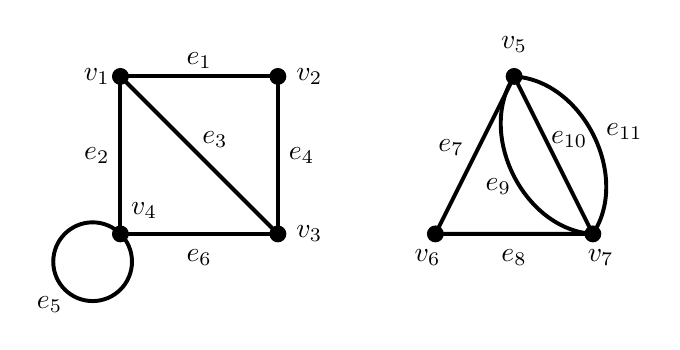
\begin{tikzpicture}
	\draw[line width= 0.05cm] (0,0) -- (2,0) -- (2,2) -- (0,2) -- (0,0);
	\draw[line width=0.05cm] (0,2) to (2,0);
	\draw[line width=0.05cm] (-0.353,-0.353) circle (0.5);
	\draw[line width=0.05cm] (4,0) -- (6,0) -- (5,2) -- (4,0);
	\draw[line width=0.05cm, bend left= 60] (6,0) to (5,2);
	\draw[line width=0.05cm, bend right= 60] (6,0) to (5,2);
	
	\draw[fill= black] (0,0) circle (0.1);
	\draw[fill= black] (2,0) circle (0.1);
	\draw[fill= black] (2,2) circle (0.1);
	\draw[fill= black] (0,2) circle (0.1);
	\draw[fill= black] (4,0) circle (0.1);
	\draw[fill= black] (6,0) circle (0.1);
	\draw[fill= black] (5,2) circle (0.1);
	
	\node at (-0.3,2) {$v_1$};
	\node at (2.4,2) {$v_2$};
	\node at (2.4,0) {$v_3$};
	\node at (0.3,0.3) {$v_4$};
	\node at (5,2.4) {$v_5$};
	\node at (3.9,-0.3) {$v_6$};
	\node at (6.1,-0.3) {$v_7$};
	
	\node at (1,2.2) {$e_1$};
	\node at (-0.3,1) {$e_2$};
	\node at (1.2,1.2) {$e_3$};
	\node at (2.3,1) {$e_4$};
	\node at (-0.9,-0.9) {$e_5$};
	\node at (1,-0.3) {$e_6$};
	\node at (4.2,1.1) {$e_7$};
	\node at (5,-0.3) {$e_8$};
	\node at (4.8,0.6) {$e_9$};
	\node at (5.7,1.2) {$e_{10}$};
	\node at (6.4,1.3) {$e_{11}$};
	\end{tikzpicture}
	\]

\begin{enumerate}[(a)]
\item Is $G$ simple? Explain. Is $G$ a multigraph? Explain.
\item Is $G$ connected? If so, explain why. If not, explain why not and find the number of connected components.
\item Find all vertices adjacent to $v_2$. Find all edges adjacent to $e_{10}$.
\item Are there any parallel edges? If not, explain why. If so, find them. 
\item Find the degrees of vertices $v_1$, $v_4$, and $v_7$. What is the degree of $G$?
\end{enumerate}



% Question 7
\newpage
\question[10] Suppose $G$ is an undirected graph whose adjacency matrix is given below. 
	\[
	\begin{pmatrix}
	0 & 1 & 3 & 0 & 0 \\
	1 & 0 & 1 & 0 & 0 \\
	3 & 1 & 0 & 0 & 0 \\
	0 & 0 & 0 & 0 & 1 \\
	0 & 0 & 0 & 1 & 0 
	\end{pmatrix}
	\]
Using only the adjacency matrix of $G$, i.e. without drawing the graph of $G$, answer the following:
        \begin{enumerate}[(a)]
        \item Does $G$ have any loops? Explain.
        \item Is $G$ connected? If so, explain why. If not, find the number of connected components.
        \item Does $G$ have any multiple edges? If so, explain why and find the vertices having multiple edges between them. If not, explain why. 
        \item Find the degree of $G$.
        \item Suppose the fifth power of the adjacency matrix is given below:
		\[
		\begin{pmatrix}
		126 & 139 & 369 & 0 & 0 \\
		139 & 78 & 139 & 0 & 0 \\
		369 & 139 & 126 & 0 & 0 \\
		0 & 0 & 0 & 0 & 1 \\
		0 & 0 & 0 & 1 & 0 
		\end{pmatrix}
		\]
	Find the number of walks of length five between $v_2$ and $v_3$. 
        \end{enumerate}




% Question 8
\newpage
\question[10] Let $G$ be the graph given below.
	\[
	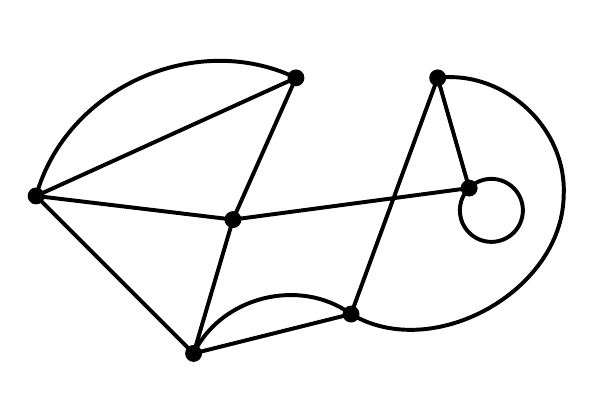
\begin{tikzpicture}
	\draw[line width=0.05cm] (0,0) -- (-2,2) -- (1.3,3.5) -- (0.5,1.7) -- (3.5,2.1) -- (3.1,3.5) -- (2,0.5) -- (0,0);
	\draw[line width=0.05cm] (-2,2) -- (0.5,1.7);
	\draw[line width=0.05cm] (0,0) -- (0.5,1.7);
	\draw[line width=0.05cm, bend left= 50] (-2,2) to (1.3,3.5);
	\draw[line width=0.05cm, bend left= 50] (0,0) to (2,0.5);
	\draw[line width=0.05cm, bend right= 60] (2,0.5) to (4.7,2);
	\draw[line width=0.05cm, bend right= 50] (4.7,2) to (3.1,3.5);
	\draw[line width=0.05cm] (3.782,1.817) circle (0.4);
	
	\draw[fill= black] (0,0) circle (0.1);
	\draw[fill= black] (2,0.5) circle (0.1);
	\draw[fill= black] (-2,2) circle (0.1);
	\draw[fill= black] (0.5,1.7) circle (0.1);
	\draw[fill= black] (3.5,2.1) circle (0.1);
	\draw[fill= black] (1.3,3.5) circle (0.1);
	\draw[fill= black] (3.1,3.5) circle (0.1);
	\end{tikzpicture}
	\]

\begin{enumerate}[(a)]
\item Does $G$ have an Eulerian circuit? If so, give an example. If not, explain why.
\item Does $G$ have an Eulerian trial? If so, give an example. If not, explain why. 
\item Does $G$ have a Hamiltonian circuit? If so, give an example. If not, explain why. 
\end{enumerate}



% Question 9
\newpage
\question[10] Suppose you have a theoretical computer with infinite memory and infinite processing power. Given an input of `size' $n$, let $A$ be an algorithm with time complexity $O(n \log n)$, $B$ be an algorithm with time complexity $O(n^2)$, and $C$ be an algorithm with time complexity $O(\sqrt{n})$. 
	\begin{enumerate}[(a)]
	\item What is the time complexity of running $A$ and $B$ in parallel? What is the time complexity of running $A$ and $C$ in parallel?
	\item What is the time complexity of running $A$ and $B$ sequentially? What is the time complexity of running $A$ and $B$ sequentially?
	\item Suppose that given an input of size $n$, an algorithm $D$ requires $A$ to be performed $n$ times, then $B$ is performed, and then $C$ is performed $n^2$ times. The algorithm then uses outputs from algorithms $A$, $B$, and $C$, performing an operation which runs in $O(1)$ time. What is the time complexity of $D$?	
	\end{enumerate}



% Question 10
\newpage
\question[10] Assume that each addition, subtraction, multiplication, division, and \texttt{print} `costs' one flop while defining/redefining variables `cost' no flops. Suppose you have an algorithm, whose pseudocode is given below, to compute a particular sum for some given fixed $n$.

\hspace{1cm} sum = 0; \par
\hspace{1cm} i = 0; j = 0; \par
\hspace{1cm} \texttt{while}(i <= n): \par
\hspace{1.5cm}	 \texttt{while}(j <= i): \par
\hspace{2cm}	term = i\^{}2 * j + j $-$ 1; \par
\hspace{2cm}	sum = sum + term \par
\hspace{2cm}	\texttt{print}([i, j, sum]) \par
\hspace{2cm} j = j + 1; \par
\hspace{1cm} i = i + 1;

\begin{enumerate}[(a)]
\item Write the outputs of this algorithm for $n= 2$.
\item Find the total flops performing this algorithm. What is the $O$ for this algorithm?
\item (Bonus) Find sum using the smallest number of total flops for `large' $n$. 
\end{enumerate}









\end{questions}
\end{document}